\documentclass[conference]{IEEEtran}
\usepackage{amsmath,amssymb,graphicx,booktabs,url}
\usepackage[hidelinks]{hyperref}
\graphicspath{{../figures/}}
\begin{document}
\title{M20 Quadruped Reconnaissance Using Terrain Mapping and Paired-Leg Step Transfer}
\author{\IEEEauthorblockN{Arnav Saurabh Surve\quad Vihan Shripad Joshi\quad Pratik Mangesh Gaikwad}
\IEEEauthorblockA{E064 / SAP 70362400067\quad E070 / SAP 70362400086\quad E073 / SAP 70362300032\\
B.Tech Computer Science and Business Systems, SVKM's NMIMS MPSTME, Mumbai\\
MDRIIA 702CO0E012, Group 09, Academic Year 2026--2027}}
\maketitle
\begin{abstract}
Hazardous-terrain reconnaissance requires mobility and sensing to work together. We preserve the supplied M20 hybrid canine quadruped with four articulated legs, sixteen motors and seventeen meshes. Ideal rays build a true-pose-referenced terrain grid; A* navigation and contact-gated paired-leg transfer negotiate three alternating barriers and two 8 cm terrace rises. A predeclared independent experiment uses thirty trials per policy across three low-roughness strata. The integrated policy accepts 30/30 missions with both climbs and zero harmful contacts; a delayed reactive software driver accepts 0/30. Terminal goal error is 0.1064 versus 12.3103 m, with proposed-minus-baseline Welch 95\% interval $[-12.2388,-12.1691]$ m. Actual 500 Hz logs contain 4,495,972 samples, independently checked against summaries. Dimensionless payback and queue models use explicitly assumed business inputs, with a separate measured-duration capacity scenario. The large comparative separation reflects a weak baseline on this fixture; it does not establish field safety, expert-operator superiority or human workload reduction.
\end{abstract}
\begin{IEEEkeywords}
quadruped, wheeled-legged robot, terrain mapping, MuJoCo, shared autonomy, reproducibility
\end{IEEEkeywords}

\section{Problem and Contribution}
The course asks how LiDAR traversability mapping can improve unknown-terrain reconnaissance while reducing teleoperation burden and latency. The supplied README identifies M20, a hybrid robot dog, as the intended platform. We preserve its articulated legs, inertias and STL assets; wheeled travel and paired leg transfer use the same complete robot.

The industrial-yard fixture includes three alternating tall barriers, cylinders, crates, boundary geometry, low rubble and two successive 8 cm concrete terrace rises. Toxic gas, structural collapse, moving hazards and loose-debris mechanics are not simulated.

Our educational contribution is auditable map-to-transfer integration: actual rays build a measured grid; local planning docks the robot before a contact-gated paired climb; evaluation rejects false success. The comparison tests the complete policy bundle against a delayed software driver. It does not establish locomotion novelty or human workload reduction.

\begin{figure}[t]
\centering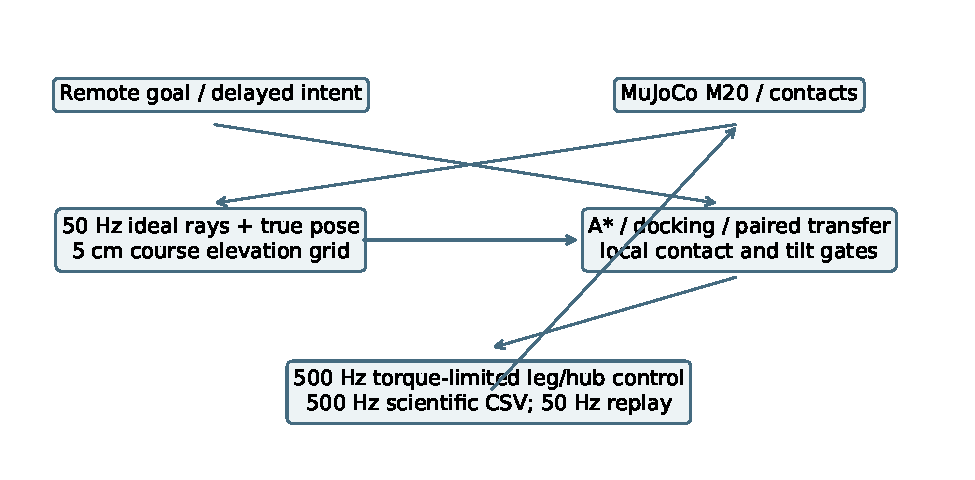
\includegraphics[width=\columnwidth]{capstone_system_architecture.pdf}
\caption{Implemented simulation pipeline. The diagram describes module flow; empirical figures below use actual MuJoCo logs. Local control can override the delayed remote-intent channel.}
\label{fig:architecture}
\end{figure}

\section{Related Work and Scope}
Fankhauser \emph{et al.} study terrain mapping with uncertain localization~\cite{fankhauser}; our simpler mapper assumes exact pose and does not propagate localization uncertainty. Di Carlo \emph{et al.} use convex model-predictive force control for quadrupeds~\cite{dicarlo}. We use an instantaneous regularized wrench allocation with clipping, without a predictive horizon or constrained MPC optimization.

Miki \emph{et al.} combine exteroception and proprioception for robust perceptive locomotion~\cite{miki}. Lee \emph{et al.} integrate learned navigation and locomotion for wheeled-legged robots~\cite{lee}. Those systems motivate platform choice and integrated control, but their learned policies and field performance are not reproduced here. Teleoperation interface and performance issues discussed by Chen \emph{et al.}~\cite{chen} motivate the delayed-driver comparison; software intervention events cannot substitute for participant workload scores. MuJoCo supplies articulated-body dynamics and contact integration~\cite{mujoco}.

\clearpage
\section{Robot and Closed-Loop Method}
\subsection{Preserved M20 Physical Model}
The model has $q\in\mathbb{R}^{23}$ generalized positions and 22 velocities: sixteen joint coordinates plus a free base represented by translation and a quaternion. Summed supplied body mass is 34.525856 kg, correcting the inherited textual value. Visual STL meshes are separate from primitive collision geometry; their collision approximation is a limitation, not a hardware-identification result. Table~\ref{tab:model} summarizes the implemented numerical model.

\begin{table}[t]
\caption{M20 model and control parameters (SI units)}\label{tab:model}
\centering\begin{tabular}{ll}\toprule
Quantity & Implemented value\\\midrule
Leg / hub actuators & 12 / 4\\
Visual meshes / mass & 17 / 34.525856 kg\\
Thigh / shank length & 0.25 / 0.25 m\\
Wheel collision / servo radius & 0.093 / 0.090 m\\
Leg / hub torque limits & 76.4 / 21.6 N m\\
Physics / torque servo & 500 / 500 Hz\\
IK and wrench allocation & 100 Hz\\
Map integration / cost update & 50 / 10 Hz\\
Dense-course grid / inflation & 0.05 / 0.70 m\\\bottomrule
\end{tabular}
\end{table}

For the sagittal two-link component, inverse kinematics uses
\begin{equation}
\cos q_k=\frac{x^2+z_{\ell}^2-l_1^2-l_2^2}{2l_1l_2},\quad l_1=l_2=0.25\ \mathrm{m}.
\end{equation}
The 0.158076 m lateral offset determines hip roll before this solve. Front and rear legs use opposite knee branches. Forward/inverse kinematics is checked against MuJoCo wheel-body positions on all four limbs.

Joint torque combines target tracking, bias compensation and stance-force terms:
\begin{equation}
\tau=\operatorname{sat}\!\left[K_p(q_d-q)-K_d\dot q+\tau_{bias}-J^Tf\right].
\end{equation}
An instantaneous allocation $f=A^T(AA^T+\lambda I)^{-1}w_d$ approximates the desired body wrench, with normal-force and friction-box clipping. It is neither a constrained contact optimum nor proof of two-foot balance. Pitch/roll state feedback and braked support hubs assist transfers. Motor commands respect supplied limits; no artificial 600 N m wheel locking is used. The floating-base state is set only for initial grounding, never rewritten to advance the robot.

\subsection{Measured Mapping and Planning}
Native multi-ray intersections exclude robot/decorative geometry by group identity, retaining genuinely tall hazards. Cells store count, mean, peak and local height variation. The true MuJoCo pose transforms the scan; this is not SLAM, ROSbot localization or a fused nine-axis inertial estimator. An interleaved scan integrates at 50 Hz simulated time, with sixteen groups requiring 0.32 s for one full lattice. Cost updates run at 10 Hz; A* requests run at 5 Hz. These are scheduling rates, not claimed wall-clock throughput.

The normalized terrain term is
\begin{equation}
c=0.4\bar{s}+0.3\bar{r}+0.3\bar{h},\quad 0\leq c\leq1,
\end{equation}
with slope, roughness and local step clipped relative to $30^\circ$, 0.04 m and 0.14 m. A separate obstacle-proximity penalty influences A*. Unknown/inflated cells are blocked, diagonal corner cuts are forbidden, and a reachable measured frontier is attempted before a no-route stop. Inflation approximates footprint plus tracking margin; it does not certify swept-volume clearance.

\begin{figure}[t]
\centering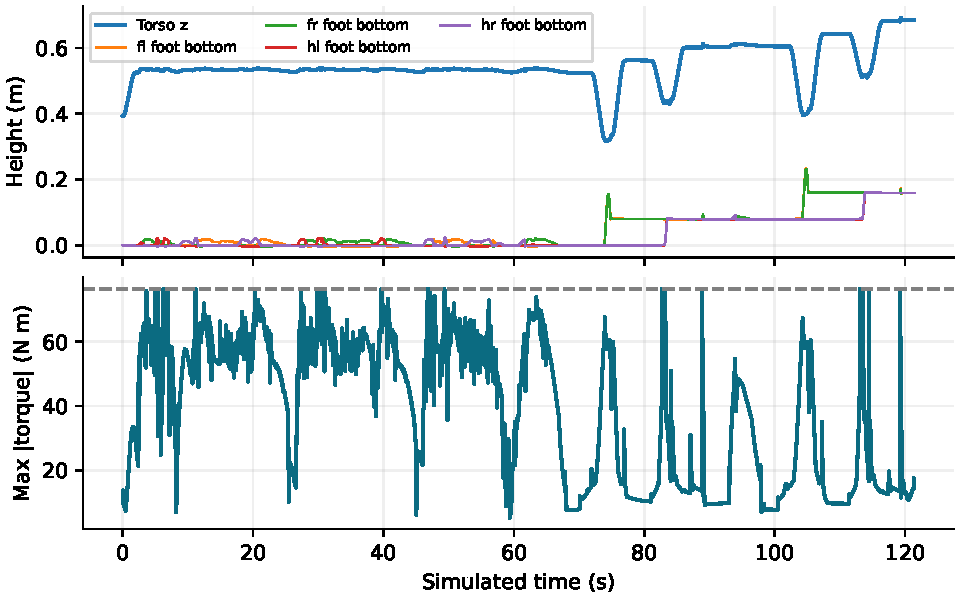
\includegraphics[width=\columnwidth]{capstone_climb_telemetry.pdf}
\caption{Actual two-climb seed-42 telemetry. Foot-bottom height subtracts the 0.093 m wheel radius; startup and two transfers are distinct. This diagnostic figure uses the 50 Hz replay channel; scientific effort uses actual 500 Hz torques.}
\label{fig:telemetry}
\end{figure}

\subsection{Paired Climb and Safety Acceptance}
A broad connected low terrace supplies a measured lip and height. The robot aligns its yaw, packs the rear stance, lowers/shifts its center of mass, swings the front pair with floating hubs, raises/pulls the torso, shifts over the front pair and swings the rear pair. Each swing transitions only after actual pair re-contact. A plateau-clearance phase precedes restoring the nominal rolling posture, avoiding premature rear-foot drop at the edge.

A verified climb requires both pair liftoffs and re-support, all four foot centers beyond the true lip, plateau-height support and base rise relative to settled standing. Terrain truth is used only by this evaluator. Goal acceptance additionally requires a 0.22 m goal region for 0.4 s, no harmful robot--world contacts, no rollover and no latched tilt stop. Wheel contacts with designated supports are expected; other world contacts are harmful and self-contact is logged separately. Contact auditing and scientific CSV logging run every 2 ms. Separate 20 ms state snapshots support replay and foot-force diagnostics.

\clearpage
\section{Experimental Design and Results}
\subsection{Independent Predeclared Protocol}
Thirty independent trials per policy compare a delayed reactive software driver with the integrated map-and-transfer executive on the same M20. The baseline has the same standing/rolling actuation but no mapper or paired climb logic. It is neither participant teleoperation nor a comparable modern planner. Policy differences bundle mapping, navigation and transfer; this is an integration comparison, not a causal single-feature ablation.

Seeds 31000--31029 and 32000--32029 are disjoint. Each arm has ten runs at each roughness bound 0, 3 and 6 mm. Nonzero rubble heights follow $U(b/2,b)$; floor friction is $U(0.75,1.15)$, barrier displacement is within $\pm0.08$ m, initial lateral position within $\pm0.02$ m and yaw within $\pm0.02$ rad. Assumed delay is 0.35 s; timeout is 180 simulated seconds. Design and source hashes were saved before execution. No outcome was sampled from a target distribution or discarded.

Every 2 ms, actual pose, velocity, sixteen torques, reference/error, FSM and contact events are saved to bounded CSV parts. A fixed evaluator-only A* polyline, computed identically for either policy from the fixture geometry, is never fed to the controller. After 2.4 s startup, nearest-segment XY error defines cross-track RMSE. This differs from timed trajectory tracking. Effort is $E=\sum_t\sum_j\tau_j^2\Delta t$; it is not energy. Unequal durations and failures affect both metrics.

\begin{table}[t]
\caption{Actual final-course outcomes, 30 runs per policy}
\centering\begin{tabular}{lrr}\toprule
Metric & Baseline & Proposed\\\midrule
Accepted / harmful-contact trials & 0 / 30 & 30 / 0\\
Rollovers & 0 & 0\\
Goal error mean (m) & 12.3103 & 0.1064\\
Goal error SD (m) & 0.0931 & 0.0082\\
Cross-track RMSE mean (m) & 0.5811 & 0.1947\\
Effort mean ($10^6$ N$^2$m$^2$s) & 1.1284 & 0.5556\\
Duration mean (s) & 180.000 & 119.731\\\bottomrule
\end{tabular}\end{table}

\subsection{Primary Inference and Interpretation}
The predeclared null is equality of mean terminal XY goal error. Independent Welch inference gives $t=-715.183$, $\nu=29.446$, $p=5.5115\times10^{-64}$. The mean difference (proposed minus baseline) is $-12.20396$ m, with 95\% interval $[-12.23884,-12.16908]$ m. Pooled-SD Cohen $d=-184.659$ is reported separately from the Welch standard error. Mann--Whitney sensitivity gives $p=3.0199\times10^{-11}$.

The enormous standardized difference arises because every baseline run stalls near the first barrier with little variability. It supports successful integration on these tasks, not general superiority or population reliability of one. Each roughness stratum has 10/10 proposed acceptance and 0/10 baseline acceptance. All baseline contacts/timeouts remain in the dataset. No normality or hardware claim follows from a small p-value.

\begin{figure}[t]\centering
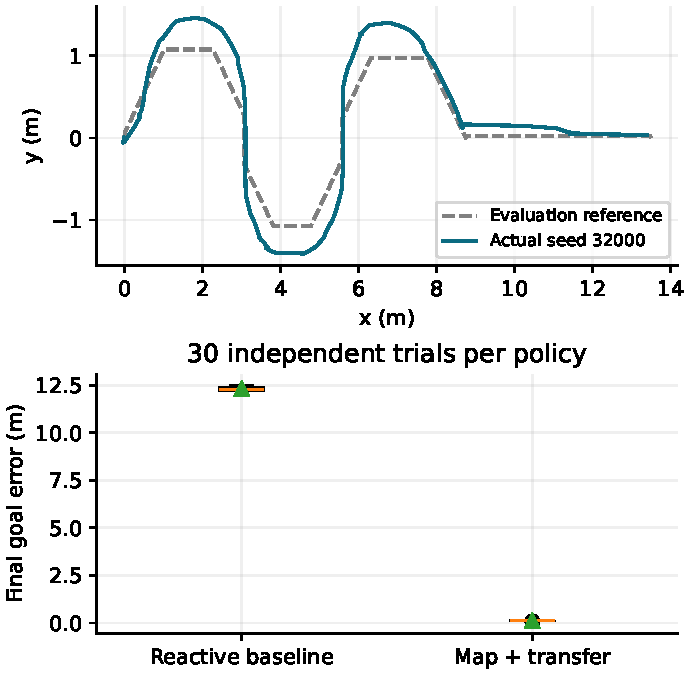
\includegraphics[width=\columnwidth]{capstone_results_paper.pdf}
\caption{Measured seed-32000 route against its fixed evaluator reference, and terminal errors for all sixty runs. Both failures and successes are retained.}\label{fig:comparison}
\end{figure}

\subsection{Reproduction and Failure Evidence}
The independent audit checks 4,495,972 samples in 254 CSV parts: SHA256, continuous 2 ms timing, run IDs/seeds, effort, RMSE, contacts, terminal distance and both pair-lift/re-support gates. Seed 42 completes both rises in 121.394 simulated seconds, with 0.107744 m goal error and no harmful contacts. Default physical states remain bitwise identical after the logger migration. Earlier 100-run, 26-run and seven-run studies remain separate, with their own protocols and source hashes.

\clearpage
\section{Operational Interpretation and Limitations}
\subsection{Dimensionless Economics and Human Factors}
All economic inputs are uncalibrated planning assumptions. With annual baseline $V=1$, operating parity $O=0.22$, capital $K=0.30$ in annual-baseline units and life $L=5$ years,
\begin{equation}
\begin{gathered}
\kappa=O/V,\qquad\mathrm{NCRI}=1-\kappa,\\
P=\frac{K}{L(V-O)},\qquad T=\frac{12K}{V-O}.
\end{gathered}
\end{equation}
Thus NCRI is 0.78, lifetime payback fraction is 0.076923 and payback is 4.615 months. Assumed 312 reclaimed hours/year gives 0.15 FTE at 2080 h/year. Scaling all cost terms equally preserves these ratios. At $V\le O$, no positive savings payback is reported; within-life break-even is $\kappa=0.94$ for the stated capital/life.

An assumed M/M/1 queue with $\lambda=8$/week, $\mu=12$/week and 40 working hours/week has $\rho=2/3$ and $W_q=\lambda/[\mu(\mu-\lambda)]=6.667$ working hours. Erlang C supports M/M/c; $\rho\ge1$ returns no finite steady-state delay. Poisson arrivals, exponential service and independence are assumptions, not observed plant processes.

A separate bridge uses actual simulation attempt duration and acceptance fraction $p$ with assumed inspection/reset overhead $h$: $\mu_{eff}=40p/(h+t/3600)$. Varying $h=1.5,3,4.5$ hours exposes the dominance of unmeasured operational work. Baseline zero accepted service yields zero scenario capacity. No NASA-TLX, bandwidth saving or observed labor benefit is inferred from motion.

\subsection{Threats to Validity}
Sensing and pose are ideal: range noise, dropout, reflective surfaces and localization drift are absent. Simulated RGB/depth panels are observational, not camera--LiDAR fusion. Robot self-exclusion uses known geometry groups. Hardware would require calibrated sensing and uncertainty-aware filtering.

Supplied meshes/inertias do not identify real hardware. Primitive collisions and rigid terraces omit tire compliance, electrical actuator dynamics, backlash, batteries and loose debris. The clipped instantaneous force allocator is not a constrained optimum. A short earlier walking check does not prove sustained braked-foot gait.

The weak reactive baseline lacks mapping and climbing. Stronger baselines and factorial ablations are required to attribute causal benefit. Thirty runs per arm in three mild roughness strata do not sample arbitrary industrial environments. Unknown terrain means no preloaded controller map; the evaluator knows fixture geometry. Terrace detection assumes broad, low steps aligned roughly with world x. No human-workload or standards-conformity claim is made.

\section{Reproducibility and Conclusion}
CPython 3.12.14, MuJoCo 3.11.0 and pinned numerical/plotting dependencies were used. The submission contains original M20 assets, tests, source hashes, every benchmark trace, failure records, analysis scripts and this editable manuscript. Running \texttt{analytics/run\_capstone\_benchmark.py} executes physics; \texttt{analyze\_capstone.py} and \texttt{plot\_capstone.py} derive the statistics and plots from those logs. CSV timestamps represent simulated time, independent of wall-clock rendering speed.



The verified result is a mesh-preserving M20 quadruped pipeline that can map, detour, align and execute paired low-step transfer in the tested simulation. Its observed comparative improvement is conditional on ideal sensing, a simple software-driver baseline and small fixed scenario families. Physical deployment, robust perception, sustained locomotion, human workload and independent validation remain future work. SI x-forward/y-left/z-up conventions are used; no ISO certification or running ROS transform system is claimed.

\paragraph{Provenance and review} The supplied mechanical model is not claimed as original CAD work. Substantial AI assistance was used for implementation, experiments and drafting. Names identify the course team, not verified individual authorship of generated code. Genuine student review, commits, expert demonstration and individual viva are pending human actions. No contributions, publication acceptance or public posting have been fabricated.

\begin{thebibliography}{6}
\bibitem{fankhauser} P. Fankhauser, M. Bloesch, and M. Hutter, ``Probabilistic terrain mapping for mobile robots with uncertain localization,'' \emph{IEEE Robot. Autom. Lett.}, 2018, doi: \url{10.1109/LRA.2018.2849506}.
\bibitem{dicarlo} J. Di Carlo, P. M. Wensing, B. Katz, G. Bledt, and S. Kim, ``Dynamic locomotion in the MIT Cheetah 3 through convex model-predictive control,'' in \emph{IROS}, 2018, doi: \url{10.1109/IROS.2018.8594448}.
\bibitem{miki} T. Miki \emph{et al.}, ``Learning robust perceptive locomotion for quadrupedal robots in the wild,'' \emph{Science Robotics}, vol. 7, eabk2822, 2022, doi: \url{10.1126/scirobotics.abk2822}.
\bibitem{lee} J. Lee \emph{et al.}, ``Learning robust autonomous navigation and locomotion for wheeled-legged robots,'' \emph{Science Robotics}, vol. 9, eadi9641, 2024, doi: \url{10.1126/scirobotics.adi9641}.
\bibitem{chen} J. Y. C. Chen, E. C. Haas, and M. J. Barnes, ``Human performance issues and user interface design for teleoperated robots,'' \emph{IEEE Trans. Syst. Man Cybern. C}, 2007, doi: \url{10.1109/TSMCC.2007.905819}.
\bibitem{mujoco} E. Todorov, T. Erez, and Y. Tassa, ``MuJoCo: A physics engine for model-based control,'' in \emph{IROS}, 2012, doi: \url{10.1109/IROS.2012.6386109}.
\end{thebibliography}
\end{document}
